% updated review slides with OHDSI template
\documentclass[11pt
%,serif,marthserif
,fragile=singleslide
%%dvips
%%,draft
,xcolor=dvipsnames
]{beamer}

%% include the preamble and all setup
%% preamble setup for OHDSI beamer template
\usepackage[]{graphicx}
%% maxwidth is the original width if it is less than linewidth
%% otherwise use linewidth (to make sure the graphics do not exceed the margin)
\makeatletter
\def\maxwidth{ %
	\ifdim\Gin@nat@width>\linewidth
	\linewidth
	\else
	\Gin@nat@width
	\fi
}
\makeatother

\definecolor{fgcolor}{rgb}{0.345, 0.345, 0.345}
\newcommand{\hlnum}[1]{\textcolor[rgb]{0.686,0.059,0.569}{#1}}%
\newcommand{\hlstr}[1]{\textcolor[rgb]{0.192,0.494,0.8}{#1}}%
\newcommand{\hlcom}[1]{\textcolor[rgb]{0.678,0.584,0.686}{\textit{#1}}}%
\newcommand{\hlopt}[1]{\textcolor[rgb]{0,0,0}{#1}}%
\newcommand{\hlstd}[1]{\textcolor[rgb]{0.345,0.345,0.345}{#1}}%
\newcommand{\hlkwa}[1]{\textcolor[rgb]{0.161,0.373,0.58}{\textbf{#1}}}%
\newcommand{\hlkwb}[1]{\textcolor[rgb]{0.69,0.353,0.396}{#1}}%
\newcommand{\hlkwc}[1]{\textcolor[rgb]{0.333,0.667,0.333}{#1}}%
\newcommand{\hlkwd}[1]{\textcolor[rgb]{0.737,0.353,0.396}{\textbf{#1}}}%

\usepackage{framed}
\makeatletter
\newenvironment{kframe}{%
	\def\at@end@of@kframe{}%
	\ifinner\ifhmode%
	\def\at@end@of@kframe{\end{minipage}}%
\begin{minipage}{\columnwidth}%
	\fi\fi%
	\def\FrameCommand##1{\hskip\@totalleftmargin \hskip-\fboxsep
		\colorbox{shadecolor}{##1}\hskip-\fboxsep
		% There is no \\@totalrightmargin, so:
		\hskip-\linewidth \hskip-\@totalleftmargin \hskip\columnwidth}%
	\MakeFramed {\advance\hsize-\width
		\@totalleftmargin\z@ \linewidth\hsize
		\@setminipage}}%
{\par\unskip\endMakeFramed%
	\at@end@of@kframe}
\makeatother

\definecolor{shadecolor}{rgb}{.97, .97, .97}
\definecolor{messagecolor}{rgb}{0, 0, 0}
\definecolor{warningcolor}{rgb}{1, 0, 1}
\definecolor{errorcolor}{rgb}{1, 0, 0}
\newenvironment{knitrout}{}{} % an empty environment to be redefined in TeX

\usepackage{alltt}
\hypersetup{pdfpagemode=FullScreen}

% \mode<presentation>
% {
%   \usetheme{Warsaw}
%   \setbeamercovered{transparent}
%   % or whatever (possibly just delete it)
% }

\usepackage[english]{babel}
% or whatever

\usepackage[utf8]{inputenc}
% or whatever

\usepackage{listings}
\usepackage{times}
\usepackage{color}
\usepackage{wasysym}
\usepackage{amstext, amssymb, amsthm, amsmath,graphicx,rotating,array}
\usepackage{algorithmic,algorithm,booktabs,url,colortbl}
%\usepackage{natbib} % commented out due to weird errors
\usepackage[T1]{fontenc}
\usepackage{amsmath}

\usepackage{eso-pic}
% \usepackage[absolute,overlay]{textpos}
\usepackage{textpos}

\usepackage{tikz}
\usepackage{pgf}
%\usepackage{cancel}
\usepackage{soul}

%\usepackage{movie15}
% Or whatever. Note that the encoding and the font should match. If T1
% does not look nice, try deleting the line with the fontenc.

\newcommand{\argmax}{\operatornamewithlimits{argmax}}

\definecolorset{rgb}{}{}{darkred,0.8,0,0;darkgreen,0,0.5,0;darkblue,0,0,0.5}
\newcommand{\bm}[1]{\mathbf{#1}}

\usepackage{color}
\usepackage{ulem}
\usepackage{wrapfig}
\usepackage{algorithm}
\usepackage{algorithmic}
\usepackage{inputenc}

% START

%\definecolor{Red}{rgb}{1,0,0}
\definecolor{ohdsiblue}{rgb}{0.125,0.259,0.353} %{0.0,0.204,0.416}
\definecolor{darkgreen}{rgb}{0.1,0.6,0.1}

\definecolorset{rgb}{}{}{darkred,0.8,0,0;darkgreen,0,0.5,0;darkblue,0,0,0.5}

\definecolor{trevorblue}{rgb}{0.330, 0.484, 0.828}
\definecolor{trevoryellow}{rgb}{0.829, 0.680, 0.306}
\definecolor{yaleblue}{rgb}{0.0,0.204,0.416}

\usetheme{Boadilla}
\usecolortheme{beaver}
\usenavigationsymbolstemplate{} % no navigation symbols

\setbeamertemplate{enumerate item}[default]

\useoutertheme{infolines}

\newcommand{\myskip}{1em}

% \setbeamercolor{author in head/foot}{fg=ohdsiblue,bg=black!5}
\setbeamercolor{author in head/foot}{fg=ohdsiblue,bg=white}
\setbeamercolor{frametitle}{fg=ohdsiblue,bg=black!5}
\setbeamercolor{block title}{bg=yaleblue!10,fg=black}

\setbeamertemplate{frametitle}{%
	\vskip-1pt
	\begin{beamercolorbox}[sep=0.3cm,wd=\paperwidth]{frametitle}
		\usebeamerfont{frametitle}%
		%\vbox{}\vskip-1ex%
		\vskip-9pt
		\hskip-9pt
		\parbox{1.5cm}{%
			
\includegraphics[width=1.5cm]{figures/logo.png}
		}
		%\hskip-2em
		%\hbox{}\vskip-3em
		\strut\insertframetitle\strut\par%
		\vskip-8pt
	\end{beamercolorbox}
}

\def\Put(#1,#2)#3{\leavevmode\makebox(0,0){\put(#1,#2){#3}}}

\setbeamertemplate{footline}[text line]{%
	\hbox{\begin{beamercolorbox}[wd=\paperwidth,ht=1em,dp=1.125ex,leftskip=.3cm plus1fill,rightskip=.3cm]{author in head/foot}%
			\usebeamerfont{author in head/foot}
			\centering 
\includegraphics[width=\paperwidth,height=1em]{figures/footer.png}
			% \centering A \insertauthor \hspace{4em} \insertshortinstitute \hspace{4em} \insertshorttitle
		\end{beamercolorbox}%
} }

% \newcommand\AtPageMyUpperLeft[1]{\AtPageLowerLeft{%
% \put(\LenToUnit{0.9\paperwidth},\LenToUnit{0.9\paperheight}){#1}}}
% \AddToShipoutPictureFG{
%   \AtPageMyUpperLeft{{\includegraphics[width=1.5cm,keepaspectratio]{OHDSI_logo_only_colored}}}
% }%

% \usepackage{pgf}
% \logo{\includegraphics[height=1cm]{OHDSI_logo_only_colored}}
% \logo{\pgfputat{\pgfxy(2,2)}{\pgfbox[center,base]{\includegraphics[width=1.7cm]{OHDSI_logo_only_colored}}}}
% \logo{\pgfputat{\pgfxy(0,8)}{\pgfbox[right,base]{\includegraphics[height=1cm]{{OHDSI_logo_only_colored}}}}}
%\logo{\pgfputat{\pgfxy(0,8)}{\pgfbox[right,base]{
\includegraphics[height=1cm]{logo.pdf}}}}
% \newcommand{\nologo}{\setbeamertemplate{logo}{}}

%\pgfdeclareimage[height=2.5cm, width=2.5cm]{logo}{OHDSI_logo_only_colored}

% \addtobeamertemplate{frametitle}{}{%
% % \begin{textblock*}{100mm}(.05\textwidth,-1cm)
% % \includegraphics[height=2cm,width=2cm]{OHDSI_logo_only_colored}
% % \end{textblock*}
% \begin{tikzpicture}[remember picture,overlay]
% \node[anchor=north west,yshift=-4pt] at (current page.north west) {\includegraphics[height=1.5cm]{OHDSI_logo_only_colored}};
% \end{tikzpicture}
% }


% \addtobeamertemplate{headline}{}
% {%
% \pgfuseimage{logo}
% % \begin{tikzpicture}[remember picture,overlay]
% % \pgfuseimage{logo}
% % \draw [line width=1mm,opacity=.25]
% % (current page.north east) circle (3cm);
% % \end{tikzpicture}
% }


% \logo{\pgfuseimage{logo}}

% END


% Delete this, if you do not want the table of contents to pop up at
% the beginning of each section:
\AtBeginSection[]
{
  \begin{frame}<beamer>
    \frametitle{Outline}
    \tableofcontents[currentsection,currentsubsection]
  \end{frame}
}


% If you wish to uncover everything in a step-wise fashion, uncomment
% the following command:

%\beamerdefaultoverlayspecification{<+->}


\setcounter{algorithm}{1}
\newcommand{\myalgorithm}[1]{
	\vspace{0.5cm}
	\begin{quote}
		{{\sc Algorithm} \arabic{algorithm}: #1}
	\end{quote}
	\vspace{1cm}
	\stepcounter{algorithm}
}

\newcommand{\HeaderA}[3]{#1 #2 #3}
\IfFileExists{upquote.sty}{\usepackage{upquote}}{}


% Specifiy title here
\title[
Bayesian Adaptive Methods Review
]
{
A First Look at the Bayesian Adaptive Methods Landscape
}
\subtitle
{} % (optional subtitle)

\author{Fan Bu}

\institute[UCLA] % (optional, but mostly needed)
{
	Departments of Human Genetics \\
	David Geffen School of Medicine at UCLA
	% - Use the \inst command only if there are several affiliations.
	% - Keep it simple, no one is interested in your street address.
}
\date{Oct 28, 2021}


% start the slides
\begin{document}
	
	\begin{frame}
		%  \titlepage
		\begin{columns}
			\begin{column}{0.33\textwidth}
				
\includegraphics[width=1.0\textwidth]{figures/logo_title_page}
			\end{column}
			\begin{column}{0.66\textwidth}
				\begin{center}
					{\LARGE
						A First Look at the Bayesian Adaptive Methods Landscape } \\[2em]
					
						Fan Bu \\[1em]
						Departments of Human Genetics \\
						David Geffen School of Medicine at UCLA
					%				}
				\end{center}
			\end{column}
		\end{columns}
		\vspace{1em}
		\vspace{1em}
		
	\end{frame}
	
	
	\begin{frame}{Overview}
		% Throughout your presentation, if you choose to use \section{} and \subsection{} commands, these will automatically be printed on this slide as an overview of your presentation
		\tableofcontents
	\end{frame}
	
	%------------------------------------------------
	\section{Basics of Bayesian hypothesis testing}
	%------------------------------------------------
	
%	\begin{frame}
%		\Huge{\centerline{Basics of Bayesian hypothesis testing}}
%	\end{frame}
	
	\begin{frame}{Basic setup}
		\begin{itemize}
			\item Observe data $X$  $ \sim p(x \mid \theta)$ (data model) with parameter $\theta$
			\item Wish to test 
			\begin{equation*}
			H_0: \theta \in \Theta_0 \qquad \text{ v.s. } \qquad H_1: \theta \in \Theta_1
			\end{equation*}
			\vspace{-0.2in}
			\pause
			\item prior beliefs about the hypotheses: 
			\begin{itemize}
				\item $p := P(H_0)$
				\item then $1-p = P(H_1)$
			\end{itemize}
			\item priors for $\theta$: $\pi_i$ under $H_i$ ($i=0,1$)
		\end{itemize}
	
	\vfill
	\rule{0.6\textwidth}{0.4pt}
	
	\footnotesize{
	Example:\\
	$x =$ EHR data; $\theta =$ safety relative risk; $p(x \mid \theta) = $ self-controlled case series model;\\
	$H_0: \theta = 0$ (same as baseline risk), $H_1: \theta > 0$ (elevated risk).
}
		
	\end{frame}
	
	\begin{frame}{Evidence checking via posterior inference}
		\begin{itemize}
			\item posterior distribution for $\theta$ under $H_i$ ($i=0,1$):
			\begin{equation*}
			p(\theta \mid x, H_i) = \frac{p(x \mid \theta) \pi_i(\theta)}{m_i(x)};
			\end{equation*}
			\item $m_i(x) = \int p(x \mid \theta) p(\theta \mid x, H_i) d\theta$: \textcolor{Cerulean}{data evidence} for $H_i$. 
			\pause
			\item posterior odds in favor of $H_0$:
			\begin{equation*}
			\frac{P(H_0 \mid x)}{P(H_1 \mid x)} = \frac{m_0(x) p}{m_1(x) (1-p)} = \frac{m_0(x)}{m_1(x)} \frac{p}{1-p};
			\end{equation*}
			\pause
			\item \textcolor{Cerulean}{Bayes factor} in favor of $H_0$ \footnote{Also the posteriors odds when $p=1/2$.}:
			\begin{equation*}
			\label{eq:bayes-factor}
			BF_{01} = \frac{m_0(x)}{m_1(x)}.
			\end{equation*}
		\end{itemize}
		
	\end{frame}
	
	\begin{frame}{Decision making}
		
		\begin{table}
			\centering
			\begin{tabular}{lll}
				\toprule
				Quantity & Threshold & Reject $H_0$ if ... \\
				\midrule
				$BF_{01}$ & $A$ ($< 1$) &   $BF_{01} < A$\\
				$P(H_0 \mid x)$ &  $\delta_L$ (small prob.) & $P(H_0 \mid x) < \delta_L$\\
				\bottomrule
			\end{tabular}
			
		\end{table}
		
%		\begin{itemize}
%%			\item For simple v.s. simple hypothesis testing, BF is same as likelihood ratio:
%%			\begin{equation*}
%%			BF_{01} = \frac{p(x \mid \theta_0)}{p(x \mid \theta_1)}.
%%			\end{equation*}
%%			\pause
%			\item With threshold $A$, reject $H_0$ if $BF_{01} < A$;
%			\item Equivalently, with threshold $\delta_L$, reject $H_0$ if $P(H_0 \mid x) < \delta_L$.
%		\end{itemize}
	
	\vfill
	\rule{0.6\textwidth}{0.4pt}
	
	\footnotesize{
		Example:\\
		If $BF_{01} < 1/10$, reject $H_0$ $\rightarrow$ claim elevated risk;\\
		Or, claim elevated risk if $P(H_0 \mid x) < 0.1$.
	}
	
	\end{frame}


%------------------------------------------------
\section{Bayesian sequential testing}
%------------------------------------------------

%\begin{frame}
%	\Huge{\centerline{Bayesian sequential testing}}
%\end{frame}

\begin{frame}{Bayesian analysis is intrinsically sequential}
	A current ``posterior'' can become the ``\textcolor{Cerulean}{prior}'' for future inference. 
	\only<1>{
		\begin{figure}
			\centering
			%\vspace{-0.1in}
			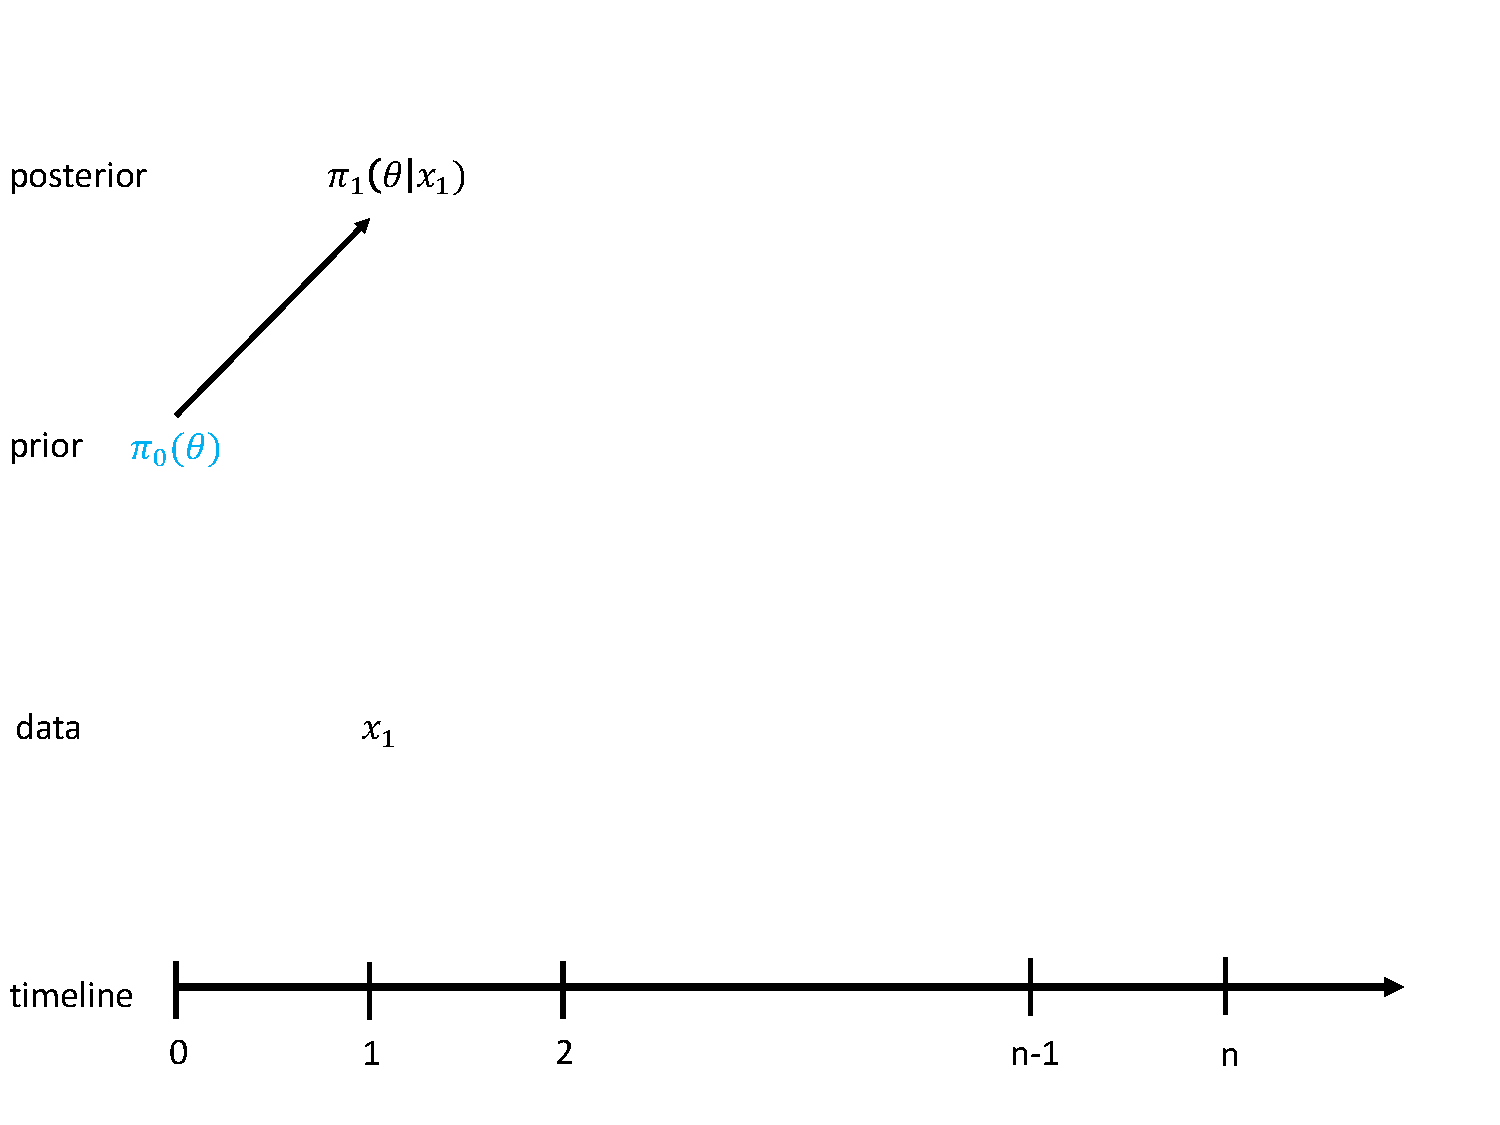
\includegraphics[width=0.82\textwidth, page=1, trim=0 0 0.5in 0.5in, clip]{figures/Bayesian_sequential_updating.pdf}
		\end{figure}
	}
	\only<2>{
		\begin{figure}
			\centering
			%\vspace{-0.1in}
			\includegraphics[width=0.82\textwidth, page=2, trim=0 0 0.5in 0.5in, clip]{figures/Bayesian_sequential_updating.pdf}
		\end{figure}
	}
%	\only<3>{
%		\begin{figure}
%			\centering
%			%\vspace{-0.1in}
%			\includegraphics[width=0.82\textwidth, page=3, trim=0 0 0.5in 0.5in, clip]{figures/Bayesian_sequential_updating.pdf}
%		\end{figure}
%	}
	\only<3>{
		\begin{figure}
			\centering
			%\vspace{-0.1in}
			\includegraphics[width=0.82\textwidth, page=4, trim=0 0 0.5in 0.5in, clip]{figures/Bayesian_sequential_updating.pdf}
		\end{figure}
	}
	
\end{frame}

\begin{frame}{How it usually works}
	Check Bayes factor $BF_{01}^{(n)}$ at step $n$ until it hits a boundary. \footnote{See, for example, \cite{barnard1946sequential,wetherill1961bayesian,berger1994unified,berger1988likelihood,berger1997unified,berger1999simultaneous}.}
%	Given thresholds $B \geq 1 \geq A$, with Bayes factor $BF_{01}^{(n)}$ acquired at step $n$ :
%	\begin{itemize}
%		\item if $BF_{01}^{(n)} > B$, stop the study and accept $H_0$;
%		\item if $A < BF_{01}^{(n)} < B$, continue the study;
%		\item  if $BF_{01}^{(n)} < A$, stop the study and reject $H_0$.
%	\end{itemize}

\begin{figure}
	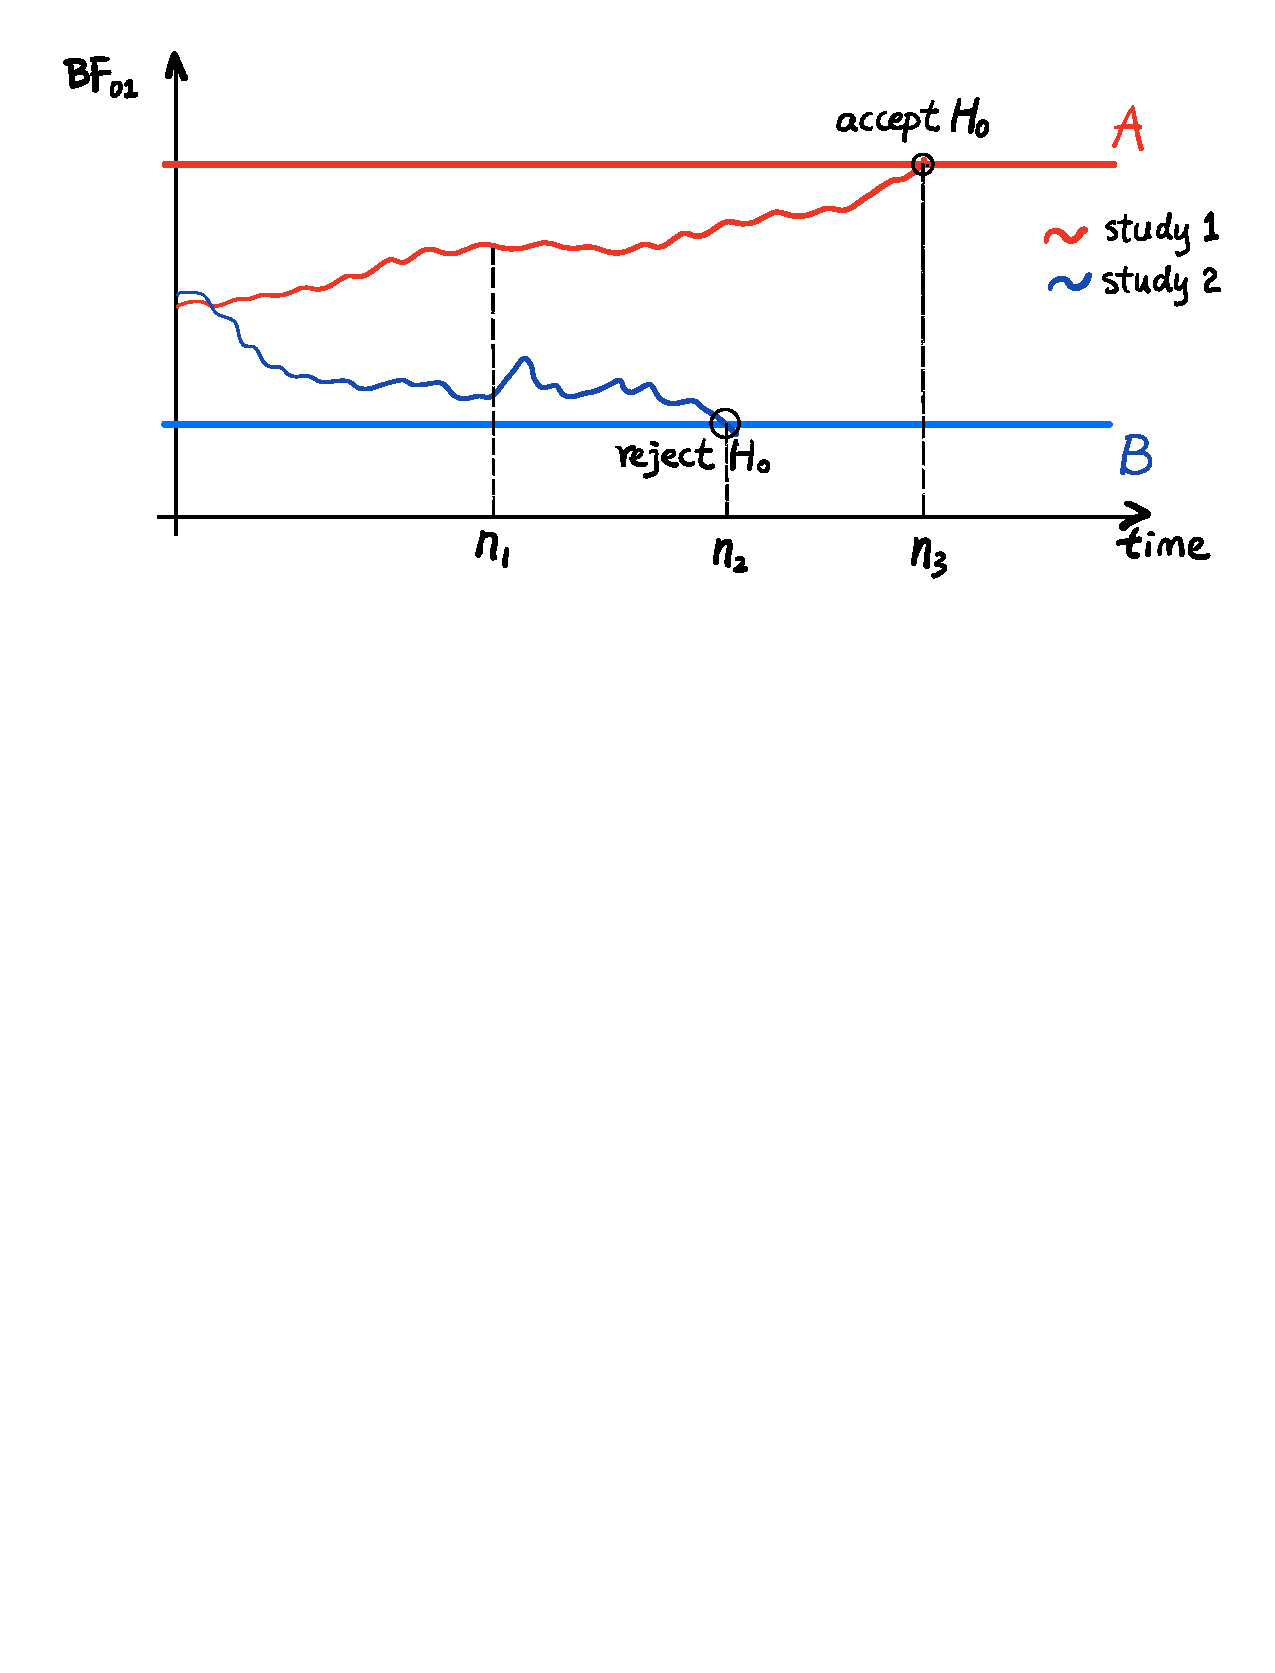
\includegraphics[width=0.83\textwidth, trim=0 7.3in 0 0.3in, clip]{figures/Bayes_Factor_Sequential_Testing.pdf}
\end{figure}
	
	\pause
	\vspace{0.15in}
	\footnotesize{
	(Can use posterior probability $P(H_0 \mid x)$ or $P(H_1 \mid x)$ too (e.g., \cite{cornfield1966bayesian}).)
}
	
\end{frame}

%------------------------------------------------
\section{Examples of Bayesian adaptive methods application}
%------------------------------------------------

%\begin{frame}
%	\Huge{Examples of Bayesian adaptive methods application}
%\end{frame}  

\begin{frame}{The setup}
	\begin{itemize}
		\item Compare effect $\theta$ with baseline $\theta_0$:
		\begin{equation*}
		H_0: \theta \leq \theta_0 \qquad \text{ v.s. } \qquad H_1: \theta > \theta_0.
		\end{equation*}
		\pause
		\item Or, consider a ``minimal practical increase'' $\delta$:
		\begin{equation*}
		H_0: \theta \leq \theta_0 + \delta \qquad \text{ v.s. } \qquad H_1: \theta > \theta_0 + \delta.
		\end{equation*}
	\end{itemize}

	\vfill
\rule{0.6\textwidth}{0.4pt}

\footnotesize{
	Example:\\
	$\theta =$ safety relative risk, $\theta_0 = 0$; \\
	$H_0$: increase 0 or negligible, $H_1$: significant elevated risk.
}
	
\end{frame}

\begin{frame}{Binary decisions}
%	\begin{itemize}
%		\item Specify lower and upper probability bounds $\delta_L$ and $\delta_U$;
%		\item \textbf{Early stopping for signal} if $P(H_1 \mid x) > \delta_U$;
%		\item \textbf{Early stopping for futility} if $P(H_1 \mid x) < \delta_L$. 
%		\item Common choice: $\delta_L = 0.05, 0.1$, $\delta_U = 0.8, 0.95$, OR calibrated through simulations.
%		
%	\end{itemize}

	\begin{table}
	\centering
	\begin{tabular}{lll}
		\toprule
		Threshold & Stop if ...  & Conclusion\\
		\midrule
		$\delta_L$ (lower) & $P(H_1 \mid x) < \delta_L$ &   futility \\
		$\delta_U$ (upper) & $P(H_1 \mid x) > \delta_U$  &  signal \\
		\bottomrule
	\end{tabular}
	
	\end{table}

\pause
\vspace{0.15in}
Common threshold choice \footnote{See, for example, \cite{thall1995bayesian,smith2006implementation,zhou2008bayesian,berry2010bayesian,li2020bayesian}, etc.}:
\begin{itemize}
	\item $\delta_L = 0.05, 0.1$; $\delta_U = 0.8, 0.95$.
	\item Or, calibrated through simulations.
\end{itemize}
	
\end{frame}

\begin{frame}{Non-binary decisions}
	
	Can give verbal labels about the \textcolor{Cerulean}{strength of evidence} in support of, e.g., $H_1$, based on  $BF_{10}$.  \cite{jeffreys1998theory,kass1995bayes,schonbrodt2017sequential}
	
	 \begin{table}
	 	\centering
	 	\begin{tabular}{ll}
	 		\toprule
	 		$BF_{10}$ range & Evidence strength in favor of $H_1$ \\
	 		\midrule
	 		$(1, 3)$ &  \textcolor{Cerulean}{anecdotal} evidence \\
	 		$(3, 10)$ &  \textcolor{Cerulean}{moderate} evidence \\
	 		$(10, 30)$ &  \textcolor{Cerulean}{strong} evidence \\
	 		$> 30$ &  \textcolor{Cerulean}{very strong} evidence\\
	 		\bottomrule
	 	\end{tabular}
	 	
	 \end{table}
	 
	%We can draw different conclusions about the strength of evidence in support of either hypothesis. 
	
%	\vspace{0.2in}
%	Decisions based on $BF_{10}$ (Bayes factor in favor of $H_1$)
%	\cite{jeffreys1998theory,kass1995bayes,schonbrodt2017sequential}:
%	\begin{itemize}
%		\item  $1 < BF_{10} < 3$: anecdotal evidence
%		\item  $3 < BF_{10} < 10$: moderate evidence
%		\item $10 <	BF_{10} < 30$: strong evidence
%		\item $BF_{10} > 30$ very strong evidence. 
%	\end{itemize}

	\vfill
\rule{0.6\textwidth}{0.4pt}

\footnotesize{
	Example:\\
	$\theta =$ safety relative risk, $\theta_0 = 0$; \\
	$H_0$: increase 0 or negligible, $H_1$: significant elevated risk.\\
	If $BF_{10} > 10$, we say ``there is strong evidence indicating a safety signal''.
}
	
\end{frame}

\begin{frame}{Non-binary decisions (Cont'd) - zone method}
	Given \textcolor{Cerulean}{indifference zone} $[\delta_L, \delta_U]$,  make decisions based on credible interval for $\Delta = \theta - \theta_0$ \cite{berry2010bayesian}. 
	
	\begin{figure}
		\centering
		%\vspace{-0.1in}
		\includegraphics[width=0.88\textwidth, page=5, trim=0 1in 0 1in, clip]{figures/Bayesian_sequential_updating.pdf}
	\end{figure}
\end{frame}
	
	
%------------------------------------------------
\section{Methodological gaps BST can address}
%------------------------------------------------

%\begin{frame}
%	\Huge{\centerline{Advantages and methodological gaps}}
%\end{frame}  

\begin{frame}{Advantages}
	\begin{itemize}
		\item Easy to incorporate \textcolor{Cerulean}{historical data} through priors.
		\only<1>{
		\begin{itemize}
			\item e.g., 10 out of 1000 subjects in historical data had an adverse event,  then can use $\text{Beta}(10,990)$ prior for incidence rate $\theta$;
			\item can \textcolor{Cerulean}{discount} prior to address temporal changes \cite{west2006bayesian}.
		\end{itemize}
	}
		\pause
		\item Can test multiple hypotheses (e.g., detect \textcolor{Cerulean}{multiple safety signals}) simultaneously. \cite{gopalan1998bayesian,berry1999bayesian,scott2006exploration,labbe2007multiple,guo2010multiplicity,kachiashvili2012sensitivity,kachiashvili2013conditional,kachiashvili2014methods,berger2013statistical}
	\end{itemize}
	
\end{frame}

\begin{frame}{Advantages}
	\begin{itemize}
		\only<1>{
		\item Can incorporate \textcolor{Cerulean}{model selection/averaging} within the Bayesian framework (e.g., \cite{raftery1995bayesian,wasserman2000bayesian,chipman2001practical,stephan2009bayesian,wathen2008bayesian,senarathne2020laplace})
	}
	\pause
		\item Non-violation of \textcolor{Cerulean}{the likelihood principle}.
%		\begin{itemize}
%			\item ``Given a statistical model, all information relavent to inferences about model parameters $\theta$ is contained in the likelihood function $L(\theta ; x)$'';
%			\item ``If two likelihood functions $L_1(\theta ; x)$ and $L_2(\theta ; x)$ are proportional then they contain same information about $\theta$''.
%			\item Conclusions about a study shouldn't depend on how we look at the data or how we decide when to stop - frequentist sequential analysis clearly violates this
%			\item Bayesian analysis respects the likelihood principle
%		\end{itemize}
	\begin{figure}
		\centering
		% commented out hand-drawing
%		\only<2>{
%		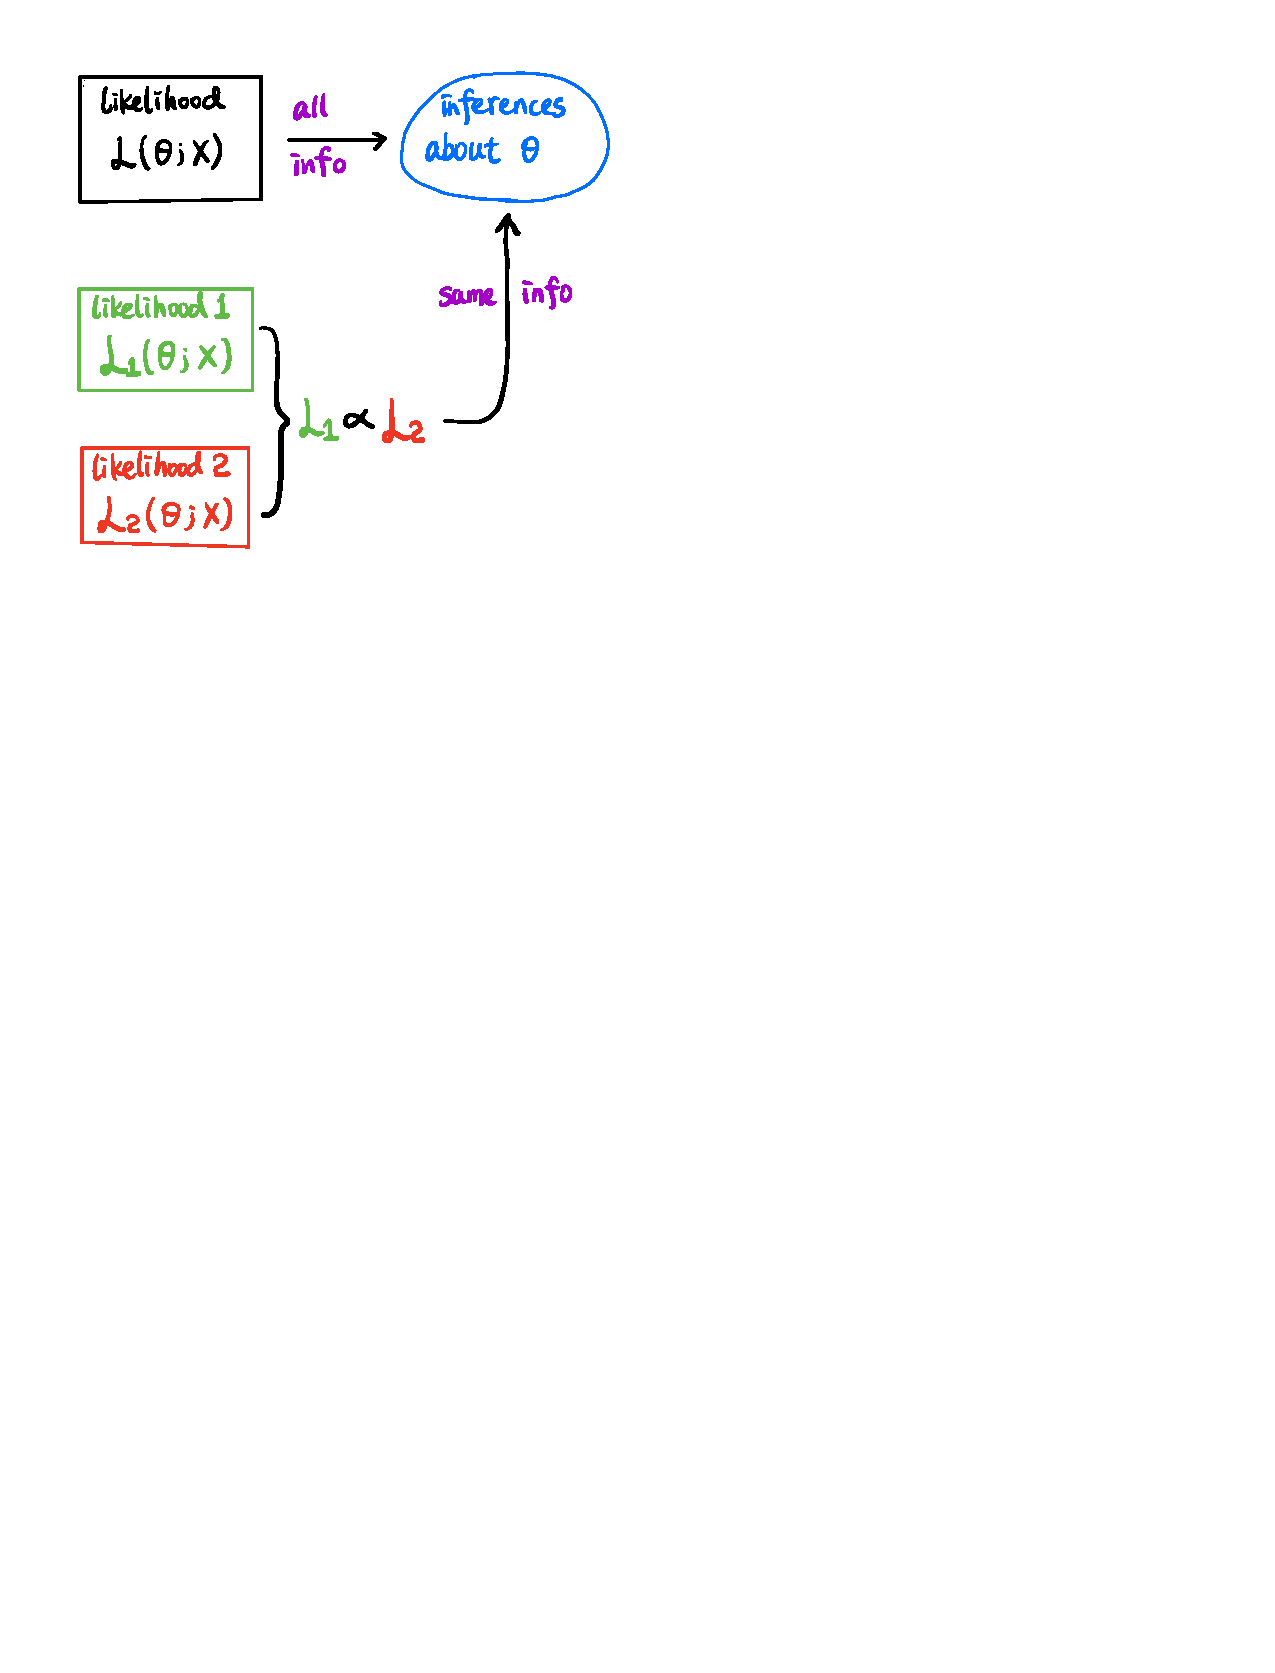
\includegraphics[width=0.85\textwidth, trim = 0.5in 3.2in 1.3in 0.2in, clip, page=1 ]{figures/Likelihood_principle_diagram.pdf}
%		}
%		\only<3>{
%			\includegraphics[width=0.85\textwidth, trim = 0.5in 3.2in 1.3in 0.2in, clip, page=2 ]{figures/Likelihood_principle_diagram.pdf}
%		}
	\only<2>{
	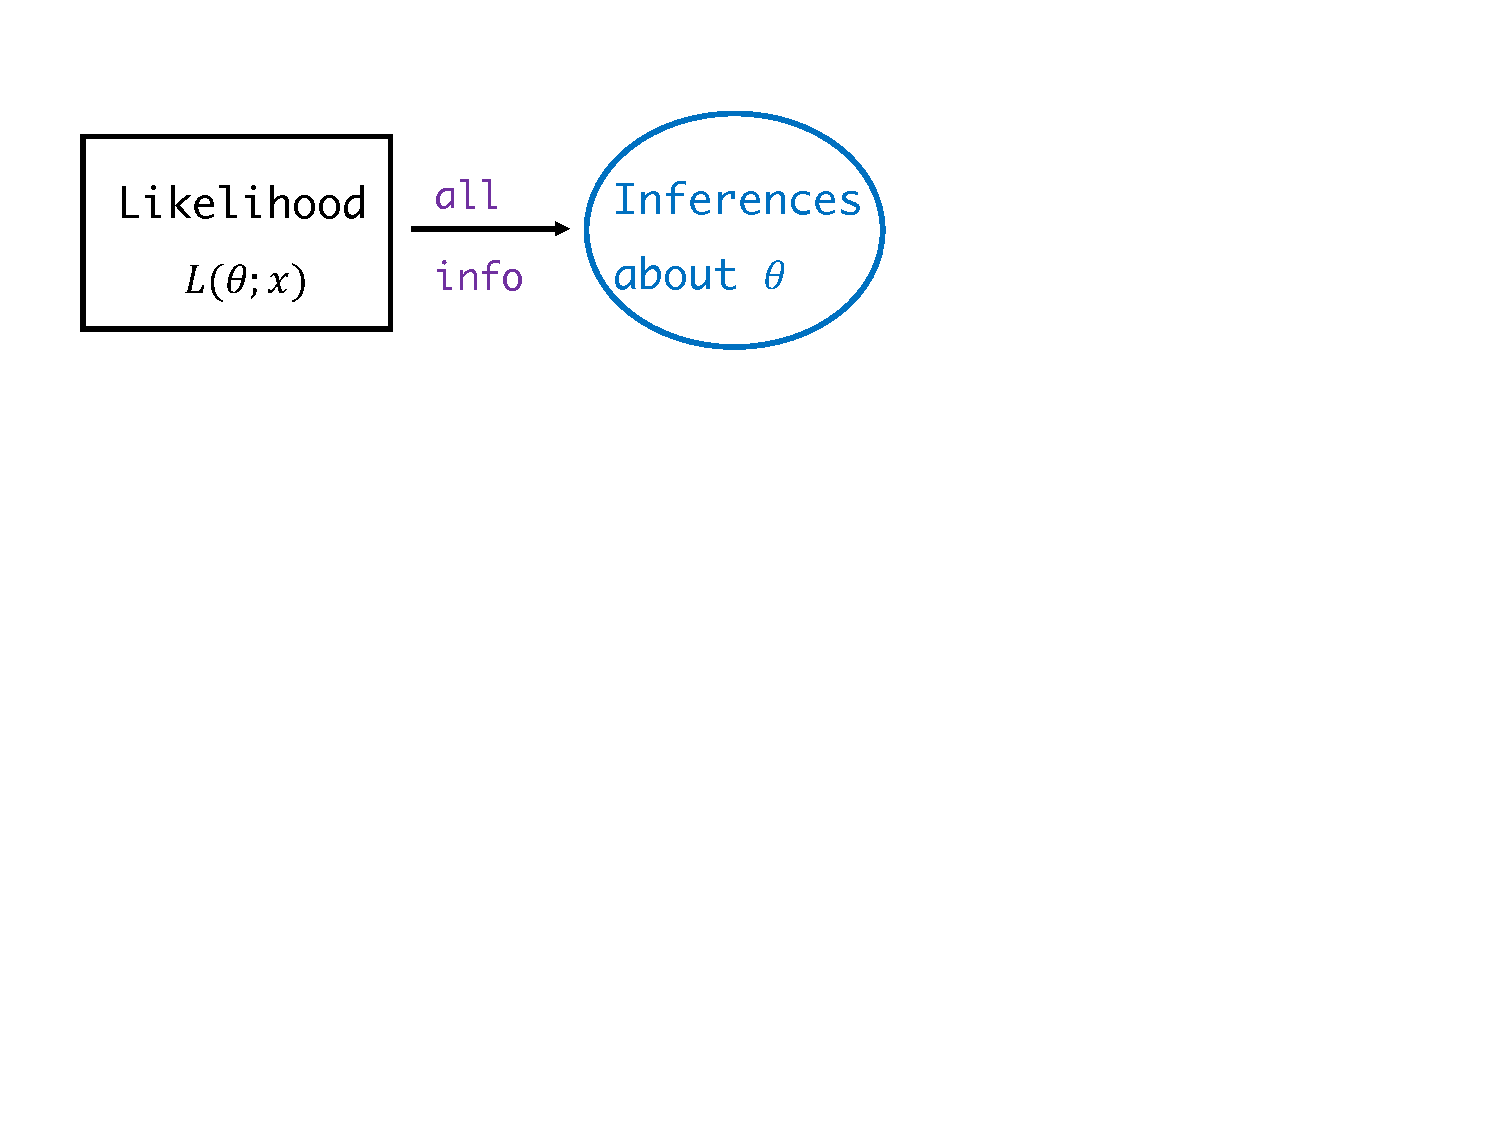
\includegraphics[width=0.82\textwidth, trim = 0.5in 0in 0in 0.5in,clip, page=1]{figures/Likelihood_principle.pdf}
	}
	\only<3>{
		\includegraphics[width=0.82\textwidth, trim = 0.5in 0in 0in 0.5in,clip, page=2]{figures/Likelihood_principle.pdf}
	}		
	\only<4>{
		\includegraphics[width=0.82\textwidth,  trim = 0.5in 0in 0in 0.5in,clip,page=3]{figures/Likelihood_principle.pdf}
	}	

	\end{figure}

	\end{itemize}
	
\end{frame}

\begin{frame}{Potential challenges}
	\begin{itemize}
		\item Calibration of the thresholds
		\begin{itemize}
			\item No universal rule (like $\alpha = 0.05$)
			\item Theoretical results available for matching frequentist error rate bounds for \textcolor{Cerulean}{simple models} (e.g.,\cite{berger1994unified, cornfield1966bayesian})
			\pause
			\item Can use simulation-based or data-driven calibration (\textcolor{Cerulean}{negative/positive controls} utilizing OHDSI network) to satisfy frequentist operating characteristics requirements 
		\end{itemize}
	\end{itemize}
	
\end{frame}

\begin{frame}{Potential challenges}
	\begin{itemize}
		\item Model-free or likelihood-free cases
		\begin{itemize}
			\item when a data model cannot be easily specified 
			\item or a likelihood function doesn't exist
			\item traditional Bayesian approach can't be applied
			\pause
			\item \textcolor{Cerulean}{generalized Bayesian} methods might be employed (e,g., \cite{turner2014generalized, lyddon2019general, bissiri2016general}).
		\end{itemize}
	\end{itemize}
	
\end{frame}


\begin{frame}
	\Huge{\centerline{Thank you!}}
\end{frame}

% Backup slides

\begin{frame}
	\Huge{\centerline{Backup slides}}
\end{frame}


\begin{frame}{An example of the likelihood principle}
	\begin{itemize}
		\item Two scientists collect binary data $X_i \sim \text{Bernoulli}(\theta)$
		\item Test $H_0: \theta = 0.5$ v.s. $H_1: \theta > 0.5$
		\item Had the same student conduct the experiment and observe $X_1, X_2, \ldots$
		\item Both decide to stop the study after collecting 12 data points
	\end{itemize}
	

\end{frame}

\begin{frame}{An example of the likelihood principle}
	\begin{columns}
		\begin{column}{0.6\textwidth}
			\begin{figure}
				\centering
				% commented out hand-drawing text
				%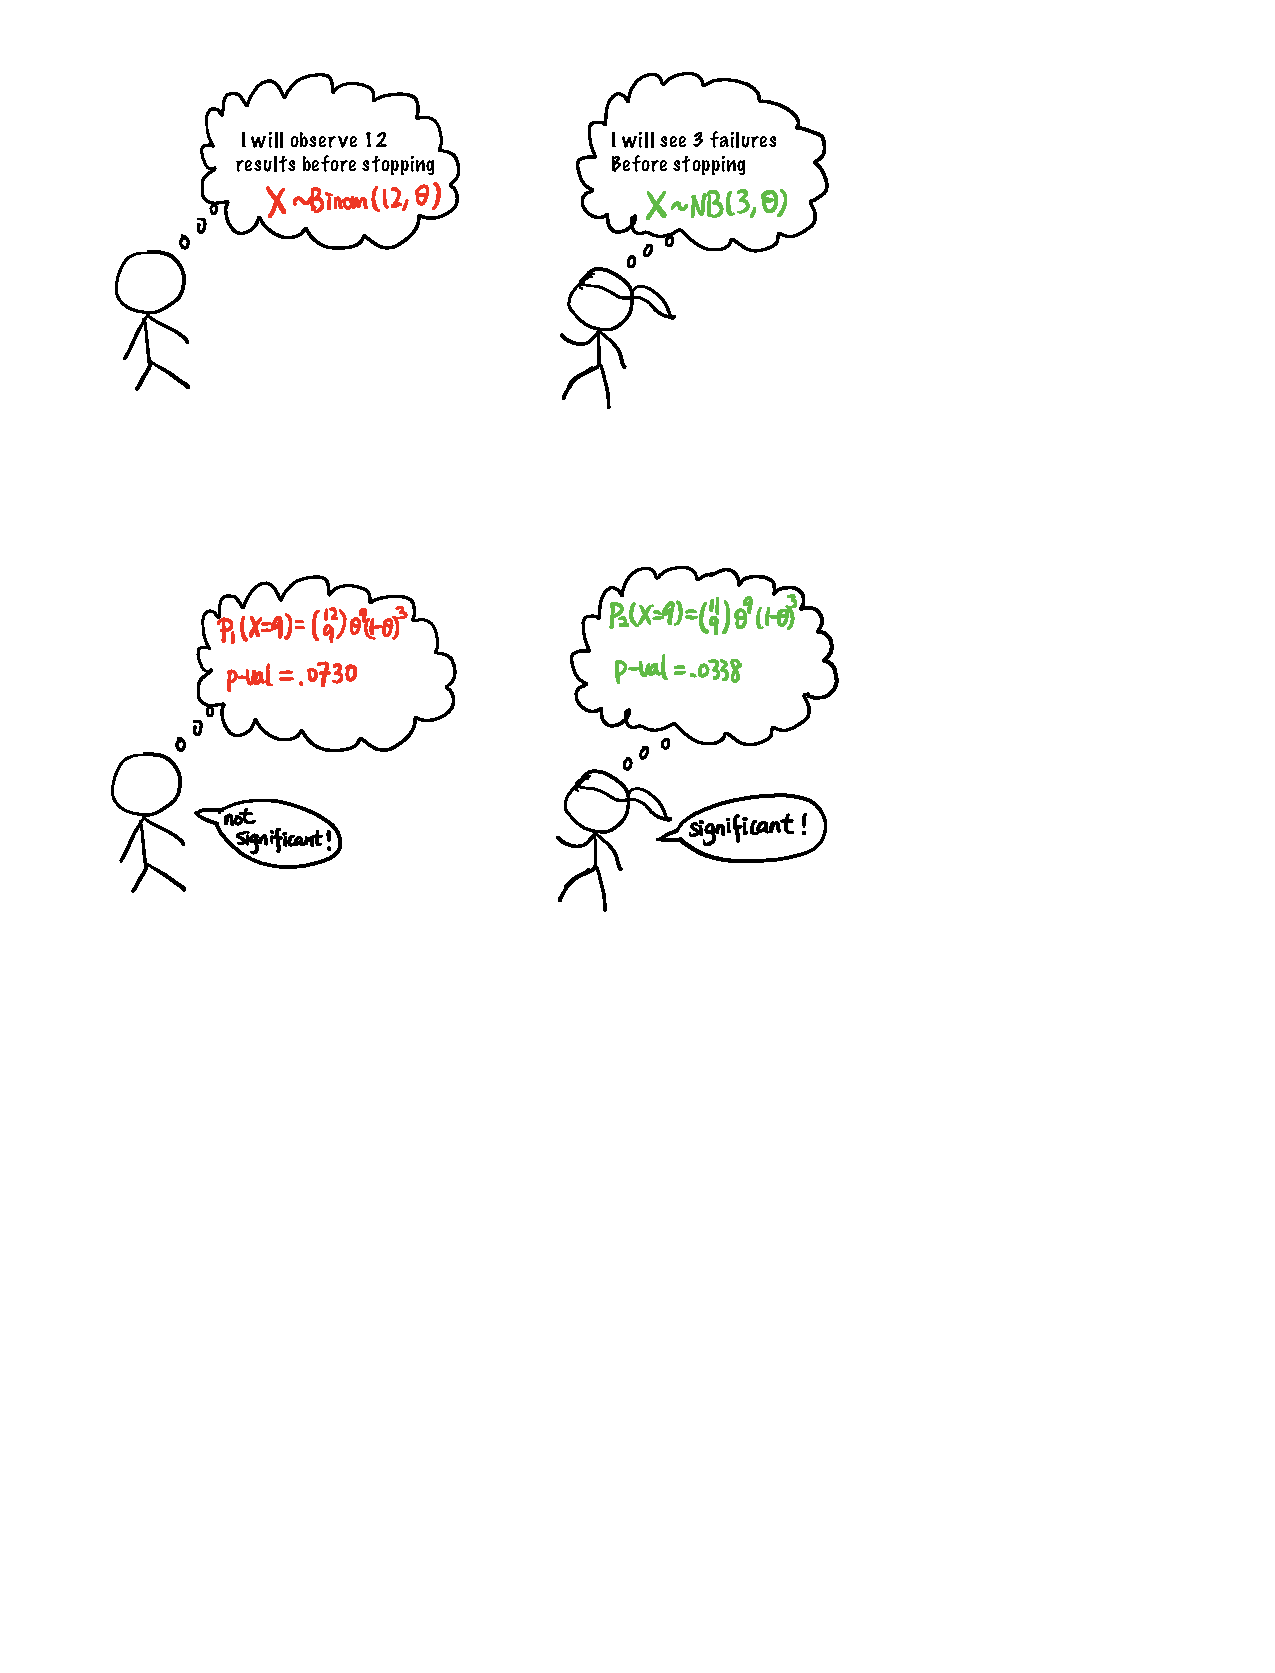
\includegraphics[width=\textwidth, trim=0 2in 2.5in 0.5in, clip]{figures/Likelihood_principle_example_1.pdf}
				\includegraphics[width=\textwidth, trim=1.3in 0in 1.5in 0in, clip, page=4]{figures/Likelihood_principle.pdf}
			\end{figure}
		\end{column}
	~
		\begin{column}{0.39\textwidth}
		\begin{itemize}
			\item They reach \textcolor{Cerulean}{different} conclusions about $\theta$
			\item Even with \textcolor{Cerulean}{proportional} likelihoods!
			\item (Both $\propto \theta^9 (1-\theta)^3$)
		\end{itemize}
		%\vspace{2.3in}
		\end{column}
		\end{columns}
\end{frame}


	
	
	% References
	\begin{frame}[allowframebreaks]
		\frametitle{References}
		\bibliographystyle{amsalpha}
		\bibliography{ref.bib}
	\end{frame}
	
	%END
	
\end{document}
